\documentclass[12pt]{article}
\setlength{\topmargin}{0in}
\setlength{\headheight}{0in}
\setlength{\headsep}{0in}
\setlength{\textheight}{8.7in}
\setlength{\textwidth}{6.5in}
\setlength{\oddsidemargin}{0in}
\setlength{\evensidemargin}{0in}
\setlength{\parindent}{0.25in}
\setlength{\parskip}{0.15in}

\special{papersize=8.5in,11in}
\setlength{\pdfpageheight}{\paperheight}
\setlength{\pdfpagewidth}{\paperwidth}

\usepackage{amsmath}
\usepackage{graphicx}

\begin{document}
\section*{Question 4}
\subsection*{Part a}
We inscribe an $N$ sided polygon into the ellipse and add up the lengths of all the sides to get an estimate for the circumference, $c$, of the ellipse.
We do this by dividing the range of $t$, (0, $2 \pi$), into $N$ equal-sized segments.
At each value of $t$ we calculate the $x$ and $y$ points on the ellipse.
For each adjacent pair of points we calculate the distance between them using Pythagoras' theorem and add them all up.

To summarise this in an equation, it is:
\begin{align}
	c = \sum_{i=1}^{N} \sqrt{\left(x(t_i) - x(t_{i-1})\right)^2 + \left(y(t_i) - y(t_{i-1})\right)^2}
\end{align}

The exact form of the circumference is actually:
\begin{align}
c = 4 a E\left(\sqrt{1 - \frac{1}{\kappa^2}}\right),
\end{align}
where $E(e)$ is the complete elliptic integral of the second kind.\footnote{I looked this up on Wikipedia}
To evaluate this I used Mathematica, as it can numerically evaluate $E(e)$ to an arbitrary number of decimal places.

To confirm the accuracy, I used $N=1000$, $a=2$, $\kappa = 2$:
\begin{align}
	c_\textnormal{me} &= 19.37686456 \\
	c_\textnormal{Mathematica} &= 19.37689644.
\end{align}
This corresponds to an accuracy of $0.0002\%$. 

\subsection*{Part b}
\begin{tabular}{c | c | c | c}
$\kappa$ & Mine & Simple & Ramanujan \\
\hline
1.0 & 12.5663 & 12.5664 & 12.5664 \\
1.3 & 14.5128 & 14.5737 & 14.5129 \\
1.6 & 16.5545 & 16.7656 & 16.5545 \\
1.9 & 18.6627 & 19.0785 & 18.6627 \\
2.2 & 20.8195 & 21.4734 & 20.8194 \\
2.5 & 23.0131 & 23.9257 & 23.0128
\end{tabular}

\subsection*{Part c}
\begin{tabular}{c | c}
$\delta$ & \\
\hline
0.00 & 18.6627 \\
0.16 & 18.6756 \\
0.32 & 18.7124 \\
0.48 & 18.7667 \\
0.64 & 18.8292 \\
0.80 & 18.8885
\end{tabular}

As $\delta$ increases, the circumference increases.
By ignoring $\delta$ this could lead to a difference of around $1\%$.

\subsection*{Part d}
See figure.
\begin{figure}
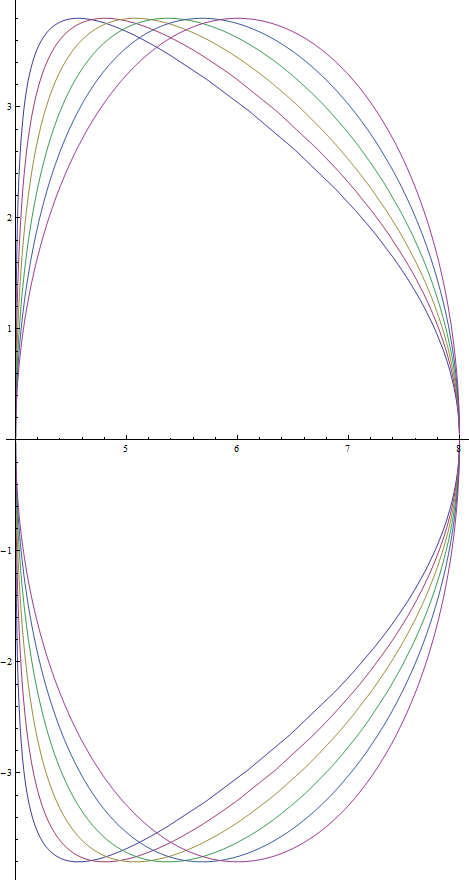
\includegraphics[width=4.5in]{ps8-q4.png}
\end{figure}

\subsection*{Part e}
For $y$ to be a maximum, the derivative must be 0:
\begin{align}
\frac{dy}{dt} = \kappa a \cos(t) &= 0 \\
\cos(t) &= 0
\end{align}
By implication this means $\sin(t) = \pm 1$.

We substitute this into our equation for $x$:
\begin{align}
x(t) &= R_0 + a \cos ( t \pm \delta ) \\
&= R_0 + a \cos(t) \cos(\delta) \mp a \sin(t) \sin(\delta) \\
&= R_0 \mp a \sin(t) \sin(\delta)
\end{align}

\end{document}